\documentclass{article}

\usepackage{graphicx}
\usepackage{subfigure}
\usepackage[hypcap]{caption}
\usepackage{listings}
\usepackage{float}
\floatstyle{plaintop}
\restylefloat{table}
\usepackage[hidelinks]{hyperref}
\usepackage[margin=1.3in]{geometry}

\title{Experimental Design and Data Analysis: \\ \large{Calcium, inorganic phosphorus and alkaline phosphatase levels\\ in elderly patients}}
\author{Andrew Bedard(2566978) \& Simone van Gompel(2567525) \\ Group 19}

\begin{document}

  \maketitle

  \section{Introduction}
  In this paper we seek to determine whether there are significant differences in the concentrations of 3 substances in the blood of elderly patients, based on gender and age groups.
    The dataset used is calcium.dat, which can be found at \url{http://www.amstat.org/publications/jse/jse_data_archive.htm}. This dataset was chosen for this project because of its reasonable size (1424 data points), and because it contained real clinical data that would give us a chance to exercise our ability to use data that likely contains errors. All tests in this paper are done with a significance value of 0.05, and the R code used is shown in the appendix.

  \section{The Experiment}
    The experiment was set up with the goal to see if age and sex has an influence on certain concentrations in the body.
    The concentrations that were measured are:
    \begin{itemize}
      \item Alkaline Phosphatase International Units/Litre (Alksphos)
      \item Calcium mmol/L (Cammol)
      \item Inorganic Phosphorus mmol/L (Phosmmol)
    \end{itemize}
    There are 6 different labs from which the data is extracted.
    Next to these features, the sex, age, age-group and patient observation number are recorded.
    In the calcium.dat the original data is stored with errors, in calciumgood.dat the data is already cleaned up, but for this paper only the calcium.dat data is considered.
    The research question we want to answer is: What influence does age and sex have on the given concentrations in the body for patients over the age of 65, and can a predictive model be created to estimate these values?

  \section{Data Analysis}
    \subsection{Preparation}
    Before loading the data into R, there were a few steps that needed to be taken. First, the table reading method in R will not work correctly if there are missing data points with no representations, so these points were manually replaced with an underscore to allow us to tell R to replace these underscores with \textit{NA}. Next headers were used to simplify our code, and let us know when we are referring to each variable by name, these were OBSNO, AGE, SEX, ALKSPHOS, LAB, CAMMOL, PHOSMMOL, AGEGRP, which represent patient number, age, sex, alkaline phosphatase in international units/litre, calcium in mmol/litre, inorganic phosphorus in mmol/litre and age group of patient respectively.
      This allowed us to create a pairs plot to get a general overview of the data, and in Fig: \ref{fig:OrgPairs}, just from observing how many points lie a great distance from the main clusters in each pair, it is clear there are a large number of outliers in our original data.

      \begin{figure}
          \centering
          {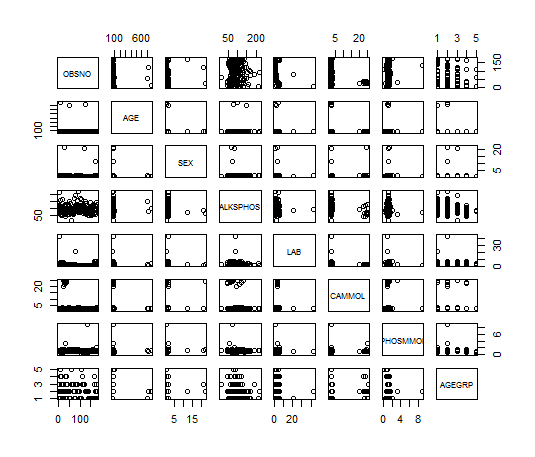
\includegraphics[scale=0.6]{../results/FirstPairs.png}\label{fig:OrgPairs}}
          \caption{Pairsplot of original data}
          \label{fig:Pairs}
      \end{figure}
      
           For example, lab 3 has strange measurements for cammol, which appears to be a misplaced decimal, causing all measurements to be an order of magnitude larger than all other measurements for cammol. This, as well as the other behaviour of the data for cammol, alksphos and phosmmol can be seen in QQ-plots of all data for each substance.(Fig: \ref{fig:qq1}) 
      \begin{figure}
		\centering
		{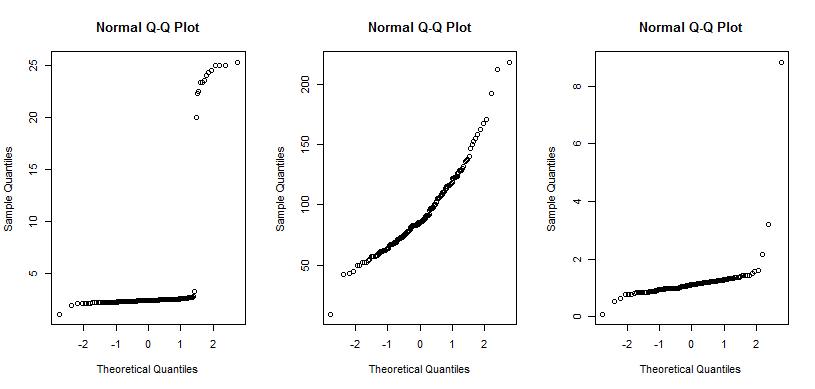
\includegraphics[scale=0.3]{../results/dat1_qq.png}}
		\caption{QQ plot of raw data, from left to right, Cammol, alksphos, phosmmol}
		\label{fig:qq1}
	\end{figure}

It is clear from Fig: \ref{fig:qq1} that our populations are certainly not normal, and this is perhaps due to the outliers. By experimentation, the values were changed in the following manner:
      \begin{itemize}
        \item Removed Ages over 110
        \item Removed Sex which is not in the category 1 or 2
        \item Removed Lab categories which are over 6
        \item Removed Phosmmol over 2 and under 0.2
        \item Divided Cammol of Lab 3 by 10 (this is visually tested by using a pairs plot)
        \item Removed Cammol over 3 and under 1.9
        \item Removed Alksphos over 150 and under 20
      \end{itemize}

Now from the Normal QQ-Plots of the transformed data Fig: \ref{fig:qq2}, we can see that we indeed have normal, or at least reasonably normal distributions. It should be noted that the stair like pattern for cammol and phosmmol concentrations are likely due to rounding.

	\begin{figure}
		\centering
		{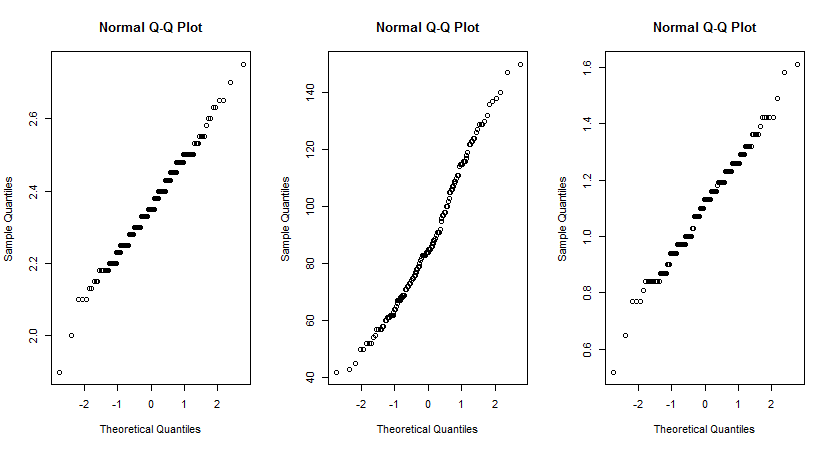
\includegraphics[scale=0.3]{../results/dat2_qq.png}}
		\caption{QQ plot after removing outliers, from left to right, Cammol, alksphos, phosmmol}
		\label{fig:qq2}
	\end{figure}
	
    \subsection{Analysis}
      The feature that needs to be analyzed is age, this can be done by either using the feature age or the feature age group.
      The age group exists of 5 levels and is thus categorical.
      The different age groups are: 1=65-69, 2=70-74, 3=75-79, 4=80-84, 5=85-89 Years.
      In Fig\ref{fig:BoxSex} the relation between the different concentrations and the sex groups are visually represented.

      \begin{figure}
          \centering
          \subfigure[Alksphos]{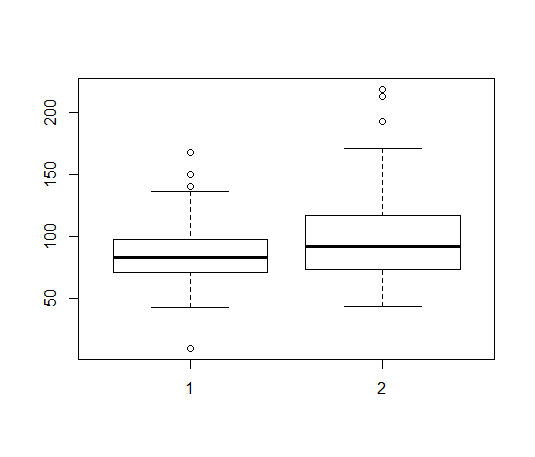
\includegraphics[scale=0.3]{../results/BoxAlksphosSex.png}}
          \subfigure[Cammol]{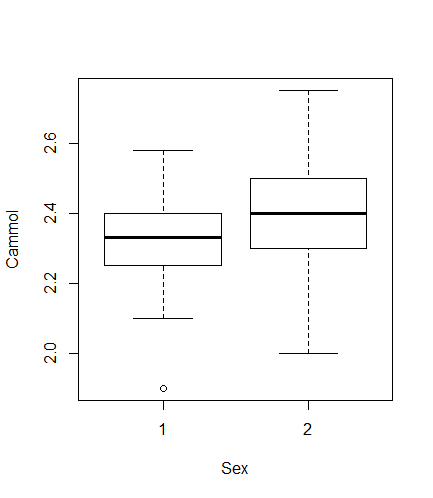
\includegraphics[scale=0.3]{../results/BoxCammolSex.png}}
          \subfigure[Phosmmol]{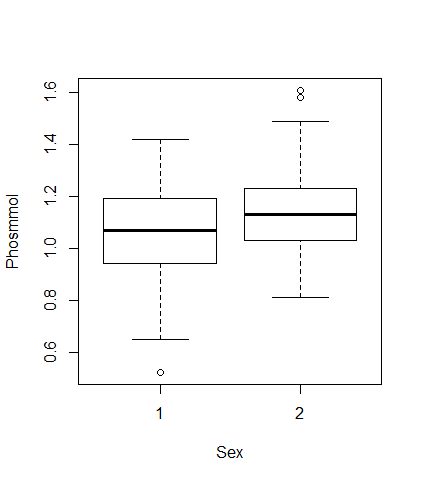
\includegraphics[scale=0.3]{../results/BoxPhosmmolSex.png}}
          \caption{Boxplots of the concentrations between sexes}
          \label{fig:BoxSex}
      \end{figure}
		
  There seems to be a subtle difference between the sexes for all concentrations, with females having slightly higher concentrations across all substances. To get a better understanding of these relationships we perform the Kruskal-Wallis rank sum test for each of our factors:Sex, Lab, and Agegrp ignoring all others, to determine whether our populations are identical across factors. The results can be seen in table: \ref{table:krusk}
  
    \begin{table}[H]
    \begin{center}
    \scriptsize
    \begin{tabular}{|ll|}
        \hline
        Variable & \textit{p} \\
        \hline 
        \hline
        CAMMOL\textasciitilde SEX & 0.001539 \\
        CAMMOL\textasciitilde LAB & 1.433e-05 \\
        CAMMOL\textasciitilde AGEGRP & 0.5451 \\
        \hline
        \hline 
        ALKSPHOS\textasciitilde SEX & 0.007631 \\
        ALKSPHOS\textasciitilde LAB & 0.001325 \\
        ALKSPHOS\textasciitilde AGEGRP & 0.6927 \\
        \hline
        \hline 
        PHOSMMOL\textasciitilde SEX & 0.007711 \\
        PHOSMMOL\textasciitilde LAB & 0.159 \\
        PHOSMMOL\textasciitilde AGEGRP & 0.006144 \\
        \hline
    \end{tabular}
    \caption{Kruskal-Wallis rank sum test}
    \label{table:krusk}
    \end{center}
    \end{table}
    
  For Cammol, we reject the null hypothesis that our populations are the same across genders and across labs.For Alksphos, we reject the null hypothesis that our populations are the same across genders and across labs, and for Phosmmol we reject the null hypothesis that our populations are the same across genders and age groups.

      The next step is to see if sex, lab and age have an influence on the concentrations while interacting with each other, the interaction plots in Fig\ref{fig:IntLabSex} and Fig\ref{fig:IntAgeSex} are made. From these plots it appears there may in fact be an interaction, though because they are parallel at times, and other times not, it makes it difficult to determine graphically if these interactions are significant, for this we use a 2-way ANOVA test, which can be seen in tables: \ref{table:AnCammol} \ref{table:AnAlsphos} \ref{table:AnPhosmmol}

      \begin{figure}[h]
          \centering
          \subfigure[Alksphos]{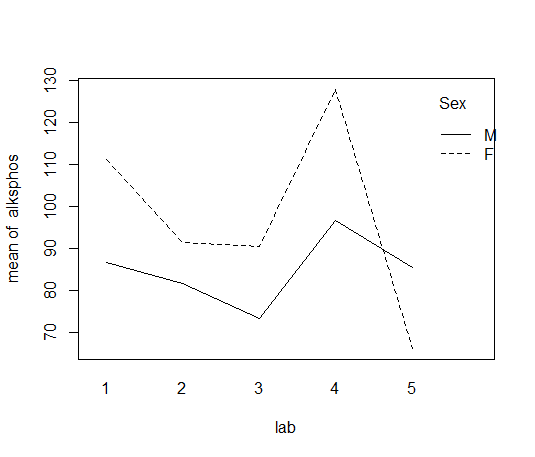
\includegraphics[scale=0.2]{../results/AlkLabSex.png}}
          \subfigure[Cammol]{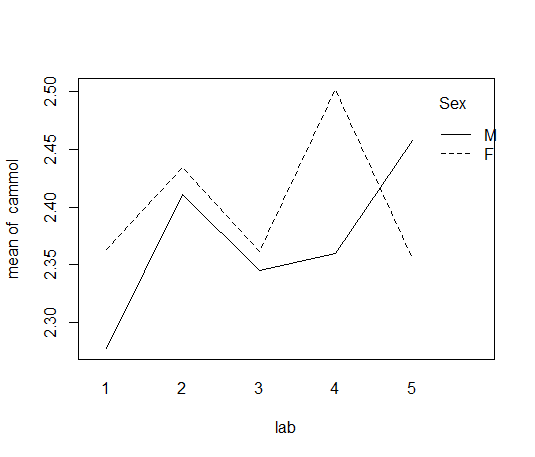
\includegraphics[scale=0.2]{../results/CamLabSex.png}}
          \subfigure[Phosmmol]{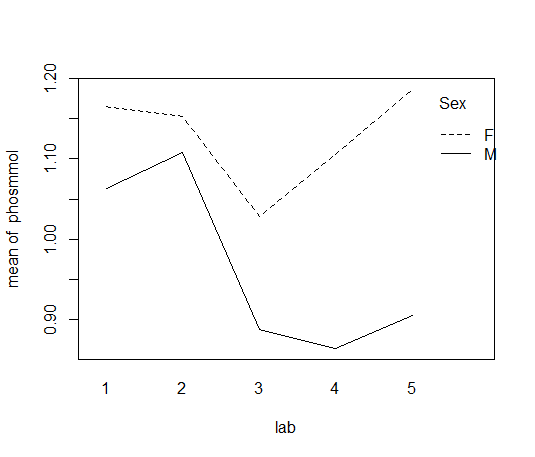
\includegraphics[scale=0.2]{../results/PhosLabSex.png}}
          \caption{Interaction plots of the sex and labs of the different concentrations}
          \label{fig:IntLabSex}
      \end{figure}
      \begin{figure}[H]
          \centering
          \subfigure[Alksphos]{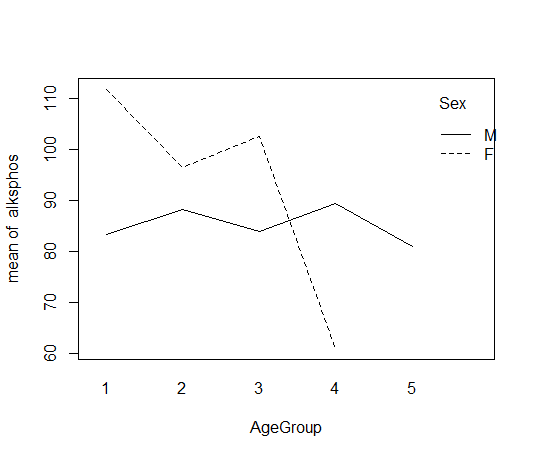
\includegraphics[scale=0.2]{../results/AlkAgeSex.png}}
          \subfigure[Cammol]{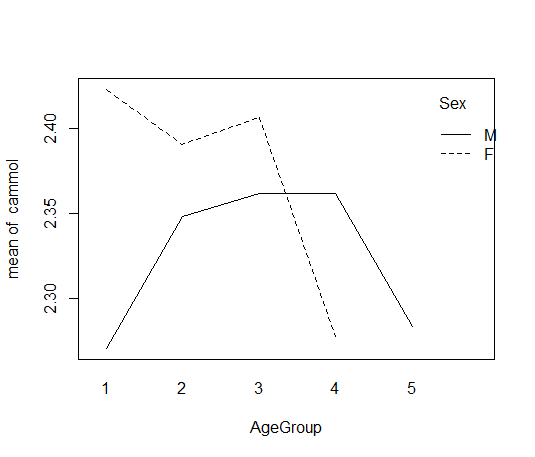
\includegraphics[scale=0.2]{../results/CamAgeSex.png}}
          \subfigure[Phosmmol]{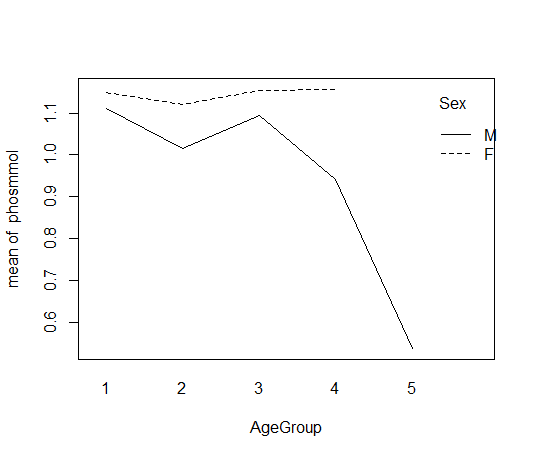
\includegraphics[scale=0.2]{../results/PhosAgeSex.png}}
          \caption{Interaction plots of the sex and age groups of the different concentrations}
          \label{fig:IntAgeSex}
      \end{figure}
      

    \begin{table}[H]
    \begin{center}
    \scriptsize
    \begin{tabular}{|l|l|l|l|}
      \hline
      $VAR1 * VAR2$:&$SEX * LAB$&$SEX * AGEGRP$&$LAB*AGEGRP$\\
      \hline
      $Var1$       & 0.00012 & 0.0003835 & 1.491e-05\\
      $Var2$       & 0.00015 & 0.9361766 & 0.4083\\
      $Var1:Var2$  & 0.51331 & 0.1214165 & 0.6595\\
      \hline
    \end{tabular}
    \caption{p-values for 2-way ANOVA, response variable: Cammol}
    \label{table:AnCammol}
    \end{center}
    \end{table}

    \begin{table}[H]
    \begin{center}
    \scriptsize
    \begin{tabular}{|l|l|l|l|}
      \hline
      $VAR1 * VAR2$:&$SEX * LAB$&$SEX * AGEGRP$&$LAB*AGEGRP$\\
      \hline
      $Var1$       & 0.05781 & 0.07838 & 0.03025\\
      $Var2$       & 0.01471 & 0.63871 & 0.72707\\
      $Var1:Var2$  & 0.53010 & 0.08933 & 0.58935\\
      \hline
    \end{tabular}
    \caption{p-values for 2-way ANOVA, response variable: Alsphos}
    \label{table:AnAlsphos}
    \end{center}
    \end{table}

    \begin{table}[H]
    \begin{center}
    \scriptsize
    \begin{tabular}{|l|l|l|l|}
      \hline
      $VAR1 * VAR2$:&$SEX * LAB$&$SEX * AGEGRP$&$LAB*AGEGRP$\\
      \hline
      $Var1$       & 0.002991 & 0.003218 & 0.18946\\
      $Var2$       & 0.006101 & 0.007732 & 0.02311\\
      $Var1:Var2$  & 0.207392 & 0.402506 & 0.16321\\
      \hline
    \end{tabular}
    \caption{p-values for 2-way ANOVA, response variable: Phosmmol}
    \label{table:AnPhosmmol}
    \end{center}
    \end{table}
 
Based on tables: \ref{table:AnCammol} \ref{table:AnAlsphos} \ref{table:AnPhosmmol}, we fail to reject the null hypothesis for all interactions between any 2 factors, thus these interactions are not in fact significant.

We further explore the QQ plots and residual plots for the linear models created to perform the 2 way ANOVA to judge the quality of our results. As we can see with both plots in Fig: \ref{fig:qq3}, there is no reason to believe that our residuals are not normal, thus our assumptions are reasonable.
    
    \begin{figure}[H]
		\centering
		\subfigure[QQ plot of residuals for all 9 linear models]
		{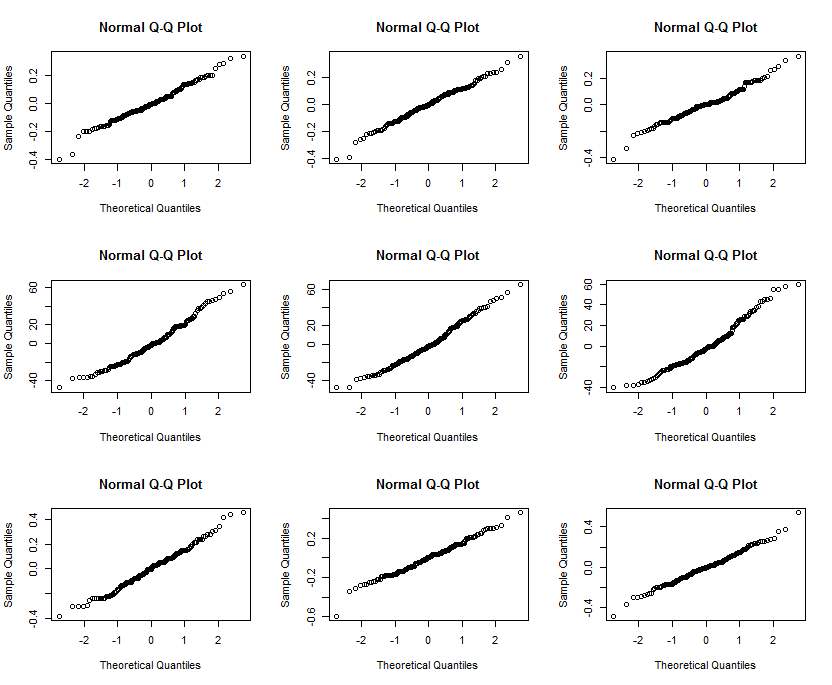
\includegraphics[scale=0.25]{../results/qq3.png}}
		\subfigure[Plots of fitted residuals for all 9 linear models]
		{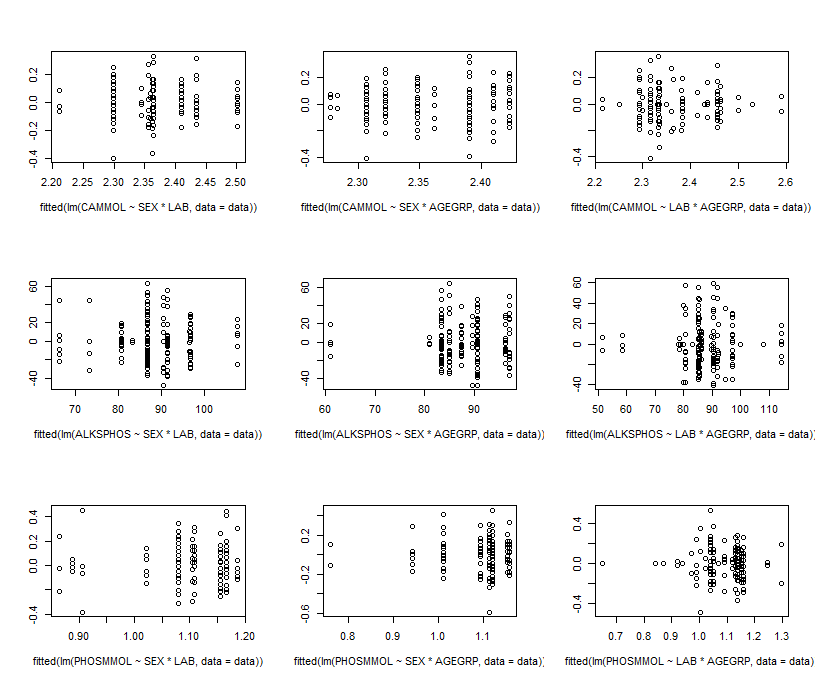
\includegraphics[scale=0.25]{../results/resid3.png}}
		\caption{Graphical tests for normality of residuals}
		\label{fig:qq3}
	\end{figure}
	
    
    \subsection{Modeling}
      Modeling the data can be done in several ways.
      The first one tried is a step down linear regression approach for each of the concentrations.
      For Alksphos it follows the following steps:
      \begin{itemize}
        \scriptsize{\item $ALKSPHOS \sim AGE + SEX + LAB + AGEGRP$}
        \scriptsize{\item $ALKSPHOS \sim AGE + SEX + LAB$}
        \scriptsize{\item $ALKSPHOS \sim SEX + LAB$}
        \scriptsize{\item $ALKSPHOS = 88.96 + 17.91*SEX2 - 11.69*LAB2 - 16.25*LAB3 + 18.03*LAB4 - 30.20*LAB5$}
      \end{itemize}
      For Cammol it follows the following steps:
      \begin{itemize}
        \scriptsize{\item $CAMMOL \sim AGE + SEX + LAB + AGEGRP$}
        \scriptsize{\item $CAMMOL \sim AGE + SEX + LAB$}
        \scriptsize{\item $CAMMOL \sim SEX + LAB$}
        \scriptsize{\item $CAMMOL = 2.29 + 0.06*SEX2 + 0.11*LAB2 + 0.03*LAB3 + 0.14*LAB4 + 0.07*LAB5$}
      \end{itemize}
      For Phosmmol it follows the following steps:
      \begin{itemize}
        \scriptsize{\item $PHOSMMOL \sim AGE + SEX + LAB + AGEGRP$}
        \scriptsize{\item $PHOSMMOL \sim AGE + SEX + LAB$}
        \scriptsize{\item $PHOSMMOL \sim AGE + SEX$}
        \scriptsize{\item $PHOSMMOL = 2.02 - 0.01*AGE + 0.17*SEX2$}
      \end{itemize}
      As our research question is about what influence age has on the concentration and only Phosmmol has a model where age was a significant explanatory variable, this is not a good approach for this data.
      
      The results of the step up model were identical, thus they shall not be considered in this paper.

  \section{Discussion}
    The data was realistic to work with as it contained many errors, likely due to human error, and at the start of the project, this was a challenge.
    The already corrected data was also supplied, but we decided against using it for the experience of working with error prone data.
    To answer our research question, does age and sex have an influence 
    The reason to not only look at age and the three concentrations was to be able to see if more features had an influence on the concentrations.
    If this was not done the results would not be correct, because the features lab and sex also had an effect on the concentrations.
    In the models created it was clear that age did not have as big an influence as first thought.
    In two of the three models, age was not included.
    This means that age has a small influence on the measured concentrations, which is the answer to our research question.
    
  \section{R-Code}
    \small{\begin{lstlisting}[language=R]
data = read.table('calcium.dat.txt', na.strings="_", header=TRUE)

# exploration
pairs(data)
par(mfrow=c(1,3))
qqnorm(data$CAMMOL)
qqnorm(data$ALKSPHOS)
qqnorm(data$PHOSMMOL)

# data preparation
data[!is.na(data$AGE) & !(data$AGE <= 110),]$AGE=NA
data[!is.na(data$SEX) & !(data$SEX == 1|data$SEX ==2),]$SEX=NA
data[!is.na(data$LAB) & !(data$LAB < 6),]$LAB=NA
data[!is.na(data$PHOSMMOL) & !(data$PHOSMMOL < 2),]$PHOSMMOL=NA
data$CAMMOL[!is.na(data$CAMMOL) & (data$CAMMOL > 10)] 
      = (data$CAMMOL[!is.na(data$CAMMOL) & (data$CAMMOL > 10)])/10
data[!is.na(data$CAMMOL) & ((data$CAMMOL < 1.9)|(data$CAMMOL >= 3)),]$CAMMOL = NA
data[!is.na(data$ALKSPHOS) & ((data$ALKSPHOS > 150)|(data$ALKSPHOS < 20)),]$ALKSPHOS
      =NA
data$SEX = as.factor(data$SEX)
data$LAB = as.factor(data$LAB)
data$AGEGRP = as.factor(data$AGEGRP)

# exploration
par(mfrow=c(1,1))
pairs(data)
par(mfrow=c(1,3))
qqnorm(data$CAMMOL)
qqnorm(data$ALKSPHOS)
qqnorm(data$PHOSMMOL)
summary(data$AGEGRP)

# data preperation, replace NA with mean
sex = data$SEX
sex[is.na(sex)]=mean(na.omit(data$SEX))
lab = data$LAB
lab[is.na(lab)]=mean(na.omit(data$LAB))
cammol = data$CAMMOL
cammol[is.na(cammol)]=mean(na.omit(data$CAMMOL))
alksphos = data$ALKSPHOS
alksphos[is.na(alksphos)]=mean(na.omit(data$ALKSPHOS))
phosmmol = data$PHOSMMOL
phosmmol[is.na(phosmmol)]=mean(na.omit(data$PHOSMMOL))

# data preperation, make sex M and F instead of 1 and 2
Sex = as.character(sex)
Sex[sex == 1] = "M"
Sex[sex == 2] = "F"
Sex = as.factor(Sex)
AgeGroup = AGEGRP

# interaction plots
par(mfrow=c(1,1))
interaction.plot(lab,Sex,cammol)
interaction.plot(lab,Sex,alksphos)
interaction.plot(lab,Sex,phosmmol)
interaction.plot(AgeGroup,Sex,cammol)
interaction.plot(AgeGroup,Sex,alksphos)
interaction.plot(AgeGroup,Sex,phosmmol)

# step down linear regression
#ALKSPHOS
summary(lm(ALKSPHOS~AGE+SEX+LAB+AGEGRP,data=data))
summary(lm(ALKSPHOS~AGE+SEX+LAB,data=data))
summary(lm(ALKSPHOS~SEX+LAB,data=data))
#CAMMOL
summary(lm(CAMMOL~AGE+SEX+LAB+AGEGRP,data=data))
summary(lm(CAMMOL~AGE+SEX+LAB,data=data))
summary(lm(CAMMOL~SEX+LAB,data=data))
#PHOSMMOL
summary(lm(PHOSMMOL~AGE+SEX+LAB+AGEGRP,data=data))
summary(lm(PHOSMMOL~AGE+SEX+LAB,data=data))
summary(lm(PHOSMMOL~AGE+SEX,data=data))

#If you looks at graphs, I dont think its fair to
#assume our data is normal. So use non-parametric test
#instead of 1 way anova
kruskal.test(CAMMOL,SEX,data=data)
kruskal.test(CAMMOL,LAB,data=data)
kruskal.test(CAMMOL,AGEGRP,data=data)

kruskal.test(ALKSPHOS,SEX,data=data)
kruskal.test(ALKSPHOS,LAB,data=data)
kruskal.test(ALKSPHOS,AGEGRP,data=data)

kruskal.test(PHOSMMOL,SEX,data=data)
kruskal.test(PHOSMMOL,LAB,data=data)
kruskal.test(PHOSMMOL,AGEGRP,data=data)

#due to difficulties with blocks being of different
#sizes we cannot use friedman test, regular 2-way 
#anova will be used.
anova(lm(CAMMOL~SEX*LAB,data=data))
anova(lm(CAMMOL~SEX*AGEGRP,data=data))
anova(lm(CAMMOL~LAB*AGEGRP,data=data))

anova(lm(ALKSPHOS~SEX*LAB,data=data))
anova(lm(ALKSPHOS~SEX*AGEGRP,data=data))
anova(lm(ALKSPHOS~LAB*AGEGRP,data=data))

anova(lm(PHOSMMOL~SEX*LAB,data=data))
anova(lm(PHOSMMOL~SEX*AGEGRP,data=data))
anova(lm(PHOSMMOL~LAB*AGEGRP,data=data))
    \end{lstlisting}}
\end{document}
